\chapter{Preprocessing}
\label{chap:preprocessing}

The exploratory analysis in Chapter~\ref{chap:data} identified several characteristics
that could bias a classifier independently of pathology: exact duplicate images,
class-specific RGB encoding, mismatched image--mask resolutions, class imbalance,
and systematic differences in global brightness and contrast. The preprocessing
strategy described here addresses these issues before model training while
preserving the original dataset and documenting every decision for reproducibility.

\section{Design Rationale}

Each preprocessing choice follows directly from the exploratory findings.
Duplicate removal prevents data leakage between training and evaluation sets.
Grayscale conversion removes the class-associated RGB encoding found in
10.41\% of Viral Pneumonia images. Mask resizing with nearest-neighbor
interpolation preserves lung boundaries when aligning $256 \times 256$ masks
with $299 \times 299$ X-rays. Stratified partitioning maintains the imbalanced
class distribution across splits. Per-image min--max normalization reduces
global intensity differences that may reflect acquisition protocol rather than
pathology. Optional contrast enhancement (CLAHE), lung-region masking, and
training-time augmentation are retained as controlled alternatives for later
comparison.

Figure~\ref{fig:preprocessing_flow} summarizes the overall workflow from the
raw collection of 21{,}165 images to the modeling-ready set of 21{,}106 samples.

\begin{figure}[H]
    \centering
    \fbox{\parbox{0.92\textwidth}{
        \small
        Raw dataset (21{,}165 images)
        $\rightarrow$ remove 59 exact duplicates
        $\rightarrow$ cleaned dataset (21{,}106 images)
        $\rightarrow$ stratified split (70\% / 15\% / 15\%)
        $\rightarrow$ per-image pipeline (grayscale, resize, optional CLAHE / lung mask / augmentation, min--max normalization)
        $\rightarrow$ training, validation, and test partitions
    }}
    \caption{End-to-end preprocessing workflow. CLAHE, lung masking, and augmentation were disabled in the baseline configuration but remain available for ablation studies.}
    \label{fig:preprocessing_flow}
\end{figure}

\section{Deduplication and Processed Dataset}

Exact duplicate groups identified during exploration yielded 59 redundant files.
These were excluded \emph{before} splitting so that identical observations cannot
appear in both training and evaluation subsets.

Table~\ref{tab:post_dedup_counts} reports the class distribution after removal.
The relative proportions remain close to the raw dataset because duplicates
represented only 0.28\% of all images and were concentrated in the COVID-19 class,
where 51 of 3{,}616 images (1.41\%) were redundant.

\begin{table}[H]
\centering
\caption{Class distribution after removing 59 exact duplicate files.}
\label{tab:post_dedup_counts}
\begin{tabular}{lrr}
\toprule
\textbf{Class} & \textbf{Images} & \textbf{Percentage} \\
\midrule
COVID-19       & 3{,}565 & 16.89\% \\
Lung Opacity   & 6{,}012 & 28.48\% \\
Normal         & 10{,}191 & 48.29\% \\
Viral Pneumonia & 1{,}338 & 6.34\% \\
\midrule
\textbf{Total} & \textbf{21{,}106} & \textbf{100.00\%} \\
\bottomrule
\end{tabular}
\end{table}

The 196 image pairs that share a perceptual hash but differ at the pixel level
were not removed automatically. They remain flagged for manual or similarity-based
review because automatic exclusion could discard legitimately distinct acquisitions.

\section{Stratified Partitioning}

The cleaned dataset was divided using a two-step stratified procedure with a
fixed random seed to ensure reproducibility:

\begin{enumerate}
    \item 70\% assigned to training and 30\% held out for evaluation.
    \item The holdout set divided equally into validation and test subsets,
    yielding an overall 70\% / 15\% / 15\% partition.
\end{enumerate}

Class proportions were preserved at each step. Table~\ref{tab:split_counts} lists
the resulting sample counts; Table~\ref{tab:split_proportions} shows that
normalized class frequencies remain aligned across all three splits, with a maximum
deviation of 0.03 percentage points for Viral Pneumonia.

\begin{table}[H]
\centering
\caption{Absolute sample counts per split after deduplication and stratification.}
\label{tab:split_counts}
\begin{tabular}{lrrrr}
\toprule
\textbf{Class} & \textbf{Train} & \textbf{Validation} & \textbf{Test} & \textbf{Total} \\
\midrule
COVID-19        & 2{,}495 & 535 & 535 & 3{,}565 \\
Lung Opacity    & 4{,}208 & 902 & 902 & 6{,}012 \\
Normal          & 7{,}134 & 1{,}528 & 1{,}529 & 10{,}191 \\
Viral Pneumonia & 937 & 201 & 200 & 1{,}338 \\
\midrule
\textbf{Total}  & \textbf{14{,}774} & \textbf{3{,}166} & \textbf{3{,}166} & \textbf{21{,}106} \\
\bottomrule
\end{tabular}
\end{table}

\begin{table}[H]
\centering
\caption{Class proportions within each split.}
\label{tab:split_proportions}
\begin{tabular}{lccc}
\toprule
\textbf{Class} & \textbf{Train} & \textbf{Validation} & \textbf{Test} \\
\midrule
COVID-19        & 16.89\% & 16.90\% & 16.90\% \\
Lung Opacity    & 28.48\% & 28.49\% & 28.49\% \\
Normal          & 48.29\% & 48.26\% & 48.29\% \\
Viral Pneumonia & 6.34\%  & 6.35\%  & 6.32\% \\
\bottomrule
\end{tabular}
\end{table}

\section{Per-Image Transformation}

Each chest X-ray underwent the following sequence of transformations.
The order matters: geometric operations precede contrast adjustment and masking,
and normalization is applied last so that intensity scaling reflects the final
pixel content presented to the model.

\begin{enumerate}
    \item \textbf{Grayscale conversion.} All images were converted to
    single-channel grayscale, eliminating the RGB encoding bias described in
    Chapter~\ref{chap:data}.

    \item \textbf{Resize.} Images were scaled to $224 \times 224$ pixels using
    area-based interpolation. Segmentation masks were resized to the same
    dimensions with nearest-neighbor interpolation to preserve binary lung
    boundaries.

    \item \textbf{Optional augmentation.} When enabled, geometric and photometric
    transforms were applied to the image and mask jointly so that spatial
    correspondence is maintained (Section~\ref{sec:augmentation}).

    \item \textbf{Optional CLAHE.} Contrast Limited Adaptive Histogram
    Equalization (clip limit 2.0, tile size $8 \times 8$) was applied to the
    image only, targeting locally varying contrast without altering mask geometry.

    \item \textbf{Optional lung masking.} Pixels outside the binarized lung
    region were zeroed before normalization, restricting intensity statistics
    to pulmonary tissue.

    \item \textbf{Per-image min--max normalization.} Each image was scaled to
    $[0, 1]$ using its own minimum and maximum pixel value:
    \[
        x' = \frac{x - x_{\min}}{x_{\max} - x_{\min} + \varepsilon},
        \qquad \varepsilon = 10^{-8}.
    \]
    Independent normalization attenuates scanner- and acquisition-specific
    global brightness differences identified in the brightness--contrast analysis.
\end{enumerate}

Figure~\ref{fig:preprocessing_transform_steps} illustrates these stages on a
representative COVID-19 chest X-ray. The aligned lung mask shows nearest-neighbor
resizing from $299 \times 299$ to $224 \times 224$. CLAHE and lung masking are
shown for illustration; both were disabled in the baseline configuration.

\begin{figure}[H]
    \centering
    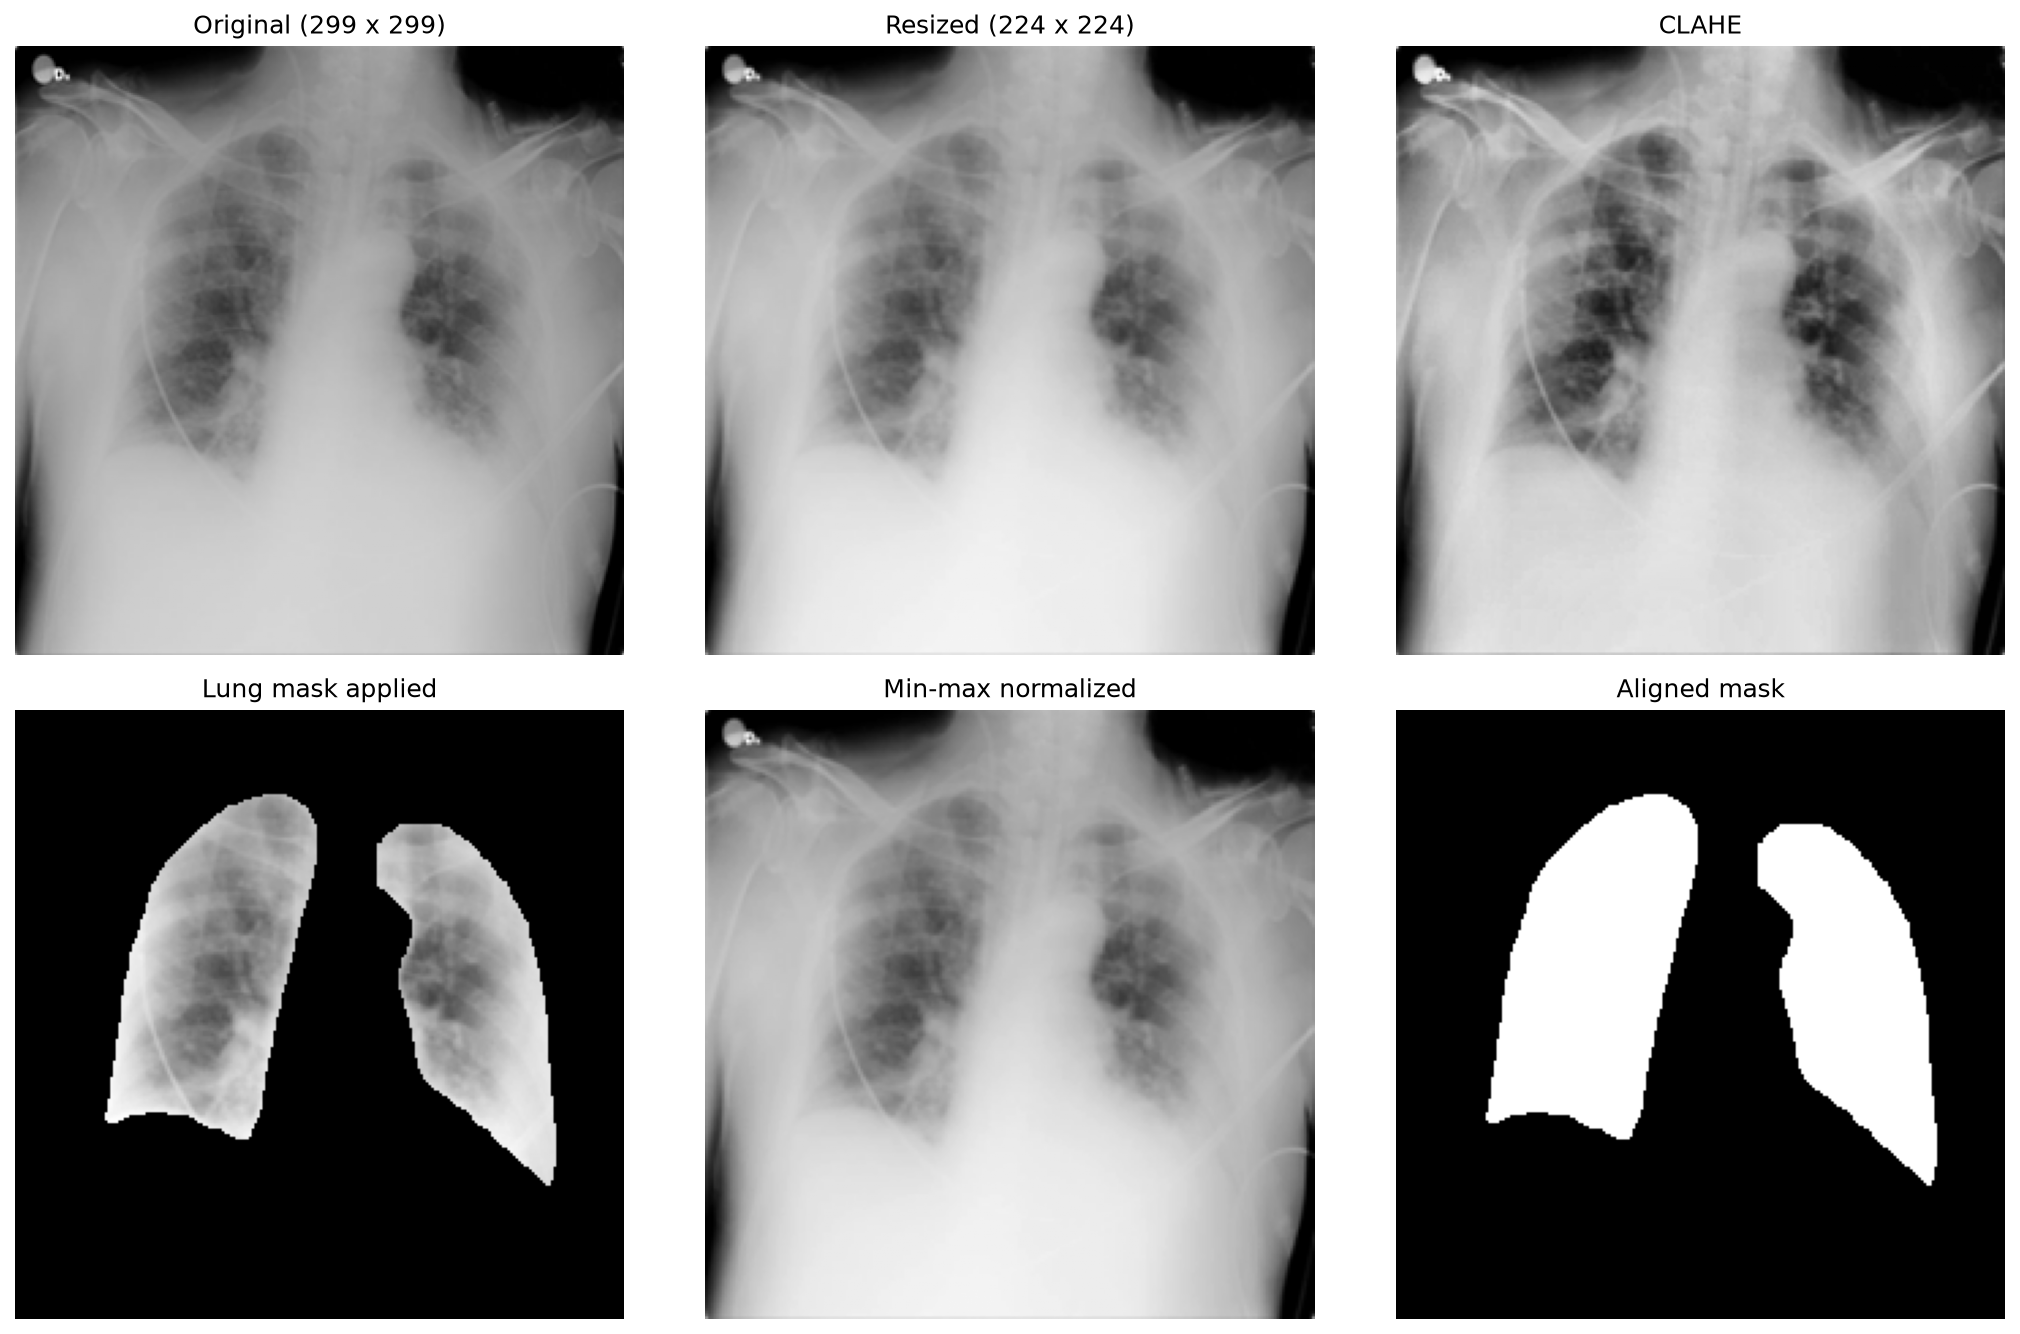
\includegraphics[width=\textwidth]{figures/preprocessing_transform_steps.png}
    \caption{Per-image preprocessing stages on a representative COVID-19 chest X-ray: original grayscale image, resize to $224 \times 224$, CLAHE, lung masking, min--max normalization, and aligned segmentation mask.}
    \label{fig:preprocessing_transform_steps}
\end{figure}

Table~\ref{tab:preprocess_defaults} summarizes the baseline configuration.
CLAHE, lung masking, and augmentation were disabled so that their effect on
downstream classification can be evaluated as controlled ablations.

\begin{table}[H]
\centering
\caption{Baseline preprocessing configuration.}
\label{tab:preprocess_defaults}
\begin{tabular}{ll}
\toprule
\textbf{Setting} & \textbf{Baseline value} \\
\midrule
Output spatial size & $224 \times 224$ pixels \\
Grayscale conversion & Applied to all images \\
CLAHE & Disabled \\
Lung mask application & Disabled \\
Lung mask binarization threshold & 127 \\
Training-time augmentation & Disabled \\
Random seed & 42 \\
Train / validation / test ratio & 70\% / 15\% / 15\% \\
\bottomrule
\end{tabular}
\end{table}

\section{Training-Time Augmentation}
\label{sec:augmentation}

Data augmentation was designed to increase effective training-set diversity
without breaking the correspondence between chest X-rays and lung segmentation
masks. Geometric transforms were applied to both modalities jointly; photometric
adjustments affected the image only. Augmentation was restricted to the training
partition so that validation and test performance reflect unmodified acquisitions.

Table~\ref{tab:augmentation} lists the operations and their activation probabilities.
Each operation is applied stochastically and independently, so a single training
sample may receive none, one, or several transforms.

\begin{table}[H]
\centering
\caption{Augmentation operations and activation probabilities.}
\label{tab:augmentation}
\begin{tabularx}{\textwidth}{llX}
\toprule
\textbf{Operation} & \textbf{Probability} & \textbf{Effect} \\
\midrule
Horizontal flip & 0.5 & Mirror image and mask about the vertical axis \\
Rotation with zoom compensation & 0.5 & Up to $\pm 15^\circ$; borders reflected on image \\
Random zoom & 0.5 & Scale change up to $\pm 8\%$; center crop or pad \\
Translation & 0.5 & Shift up to $\pm 5\%$ of width and height \\
Brightness / contrast & 0.4 & Intensity scaling up to $\pm 10\%$; image only \\
\bottomrule
\end{tabularx}
\end{table}


Rotation without zoom compensation was evaluated separately and found to introduce
empty border regions in the segmentation mask when reflect padding was used.
The zoom-compensated rotation variant scales the image to fill the frame and
uses zero padding on the mask, keeping lung labels binary. Figure~\ref{fig:preprocessing_augmentation_ops}
compares individual geometric transforms on a representative COVID-19 case.
Figure~\ref{fig:preprocessing_augment_pair} shows the combined effect of a single
stochastic augmentation pass on the same sample.

\begin{figure}[H]
    \centering
    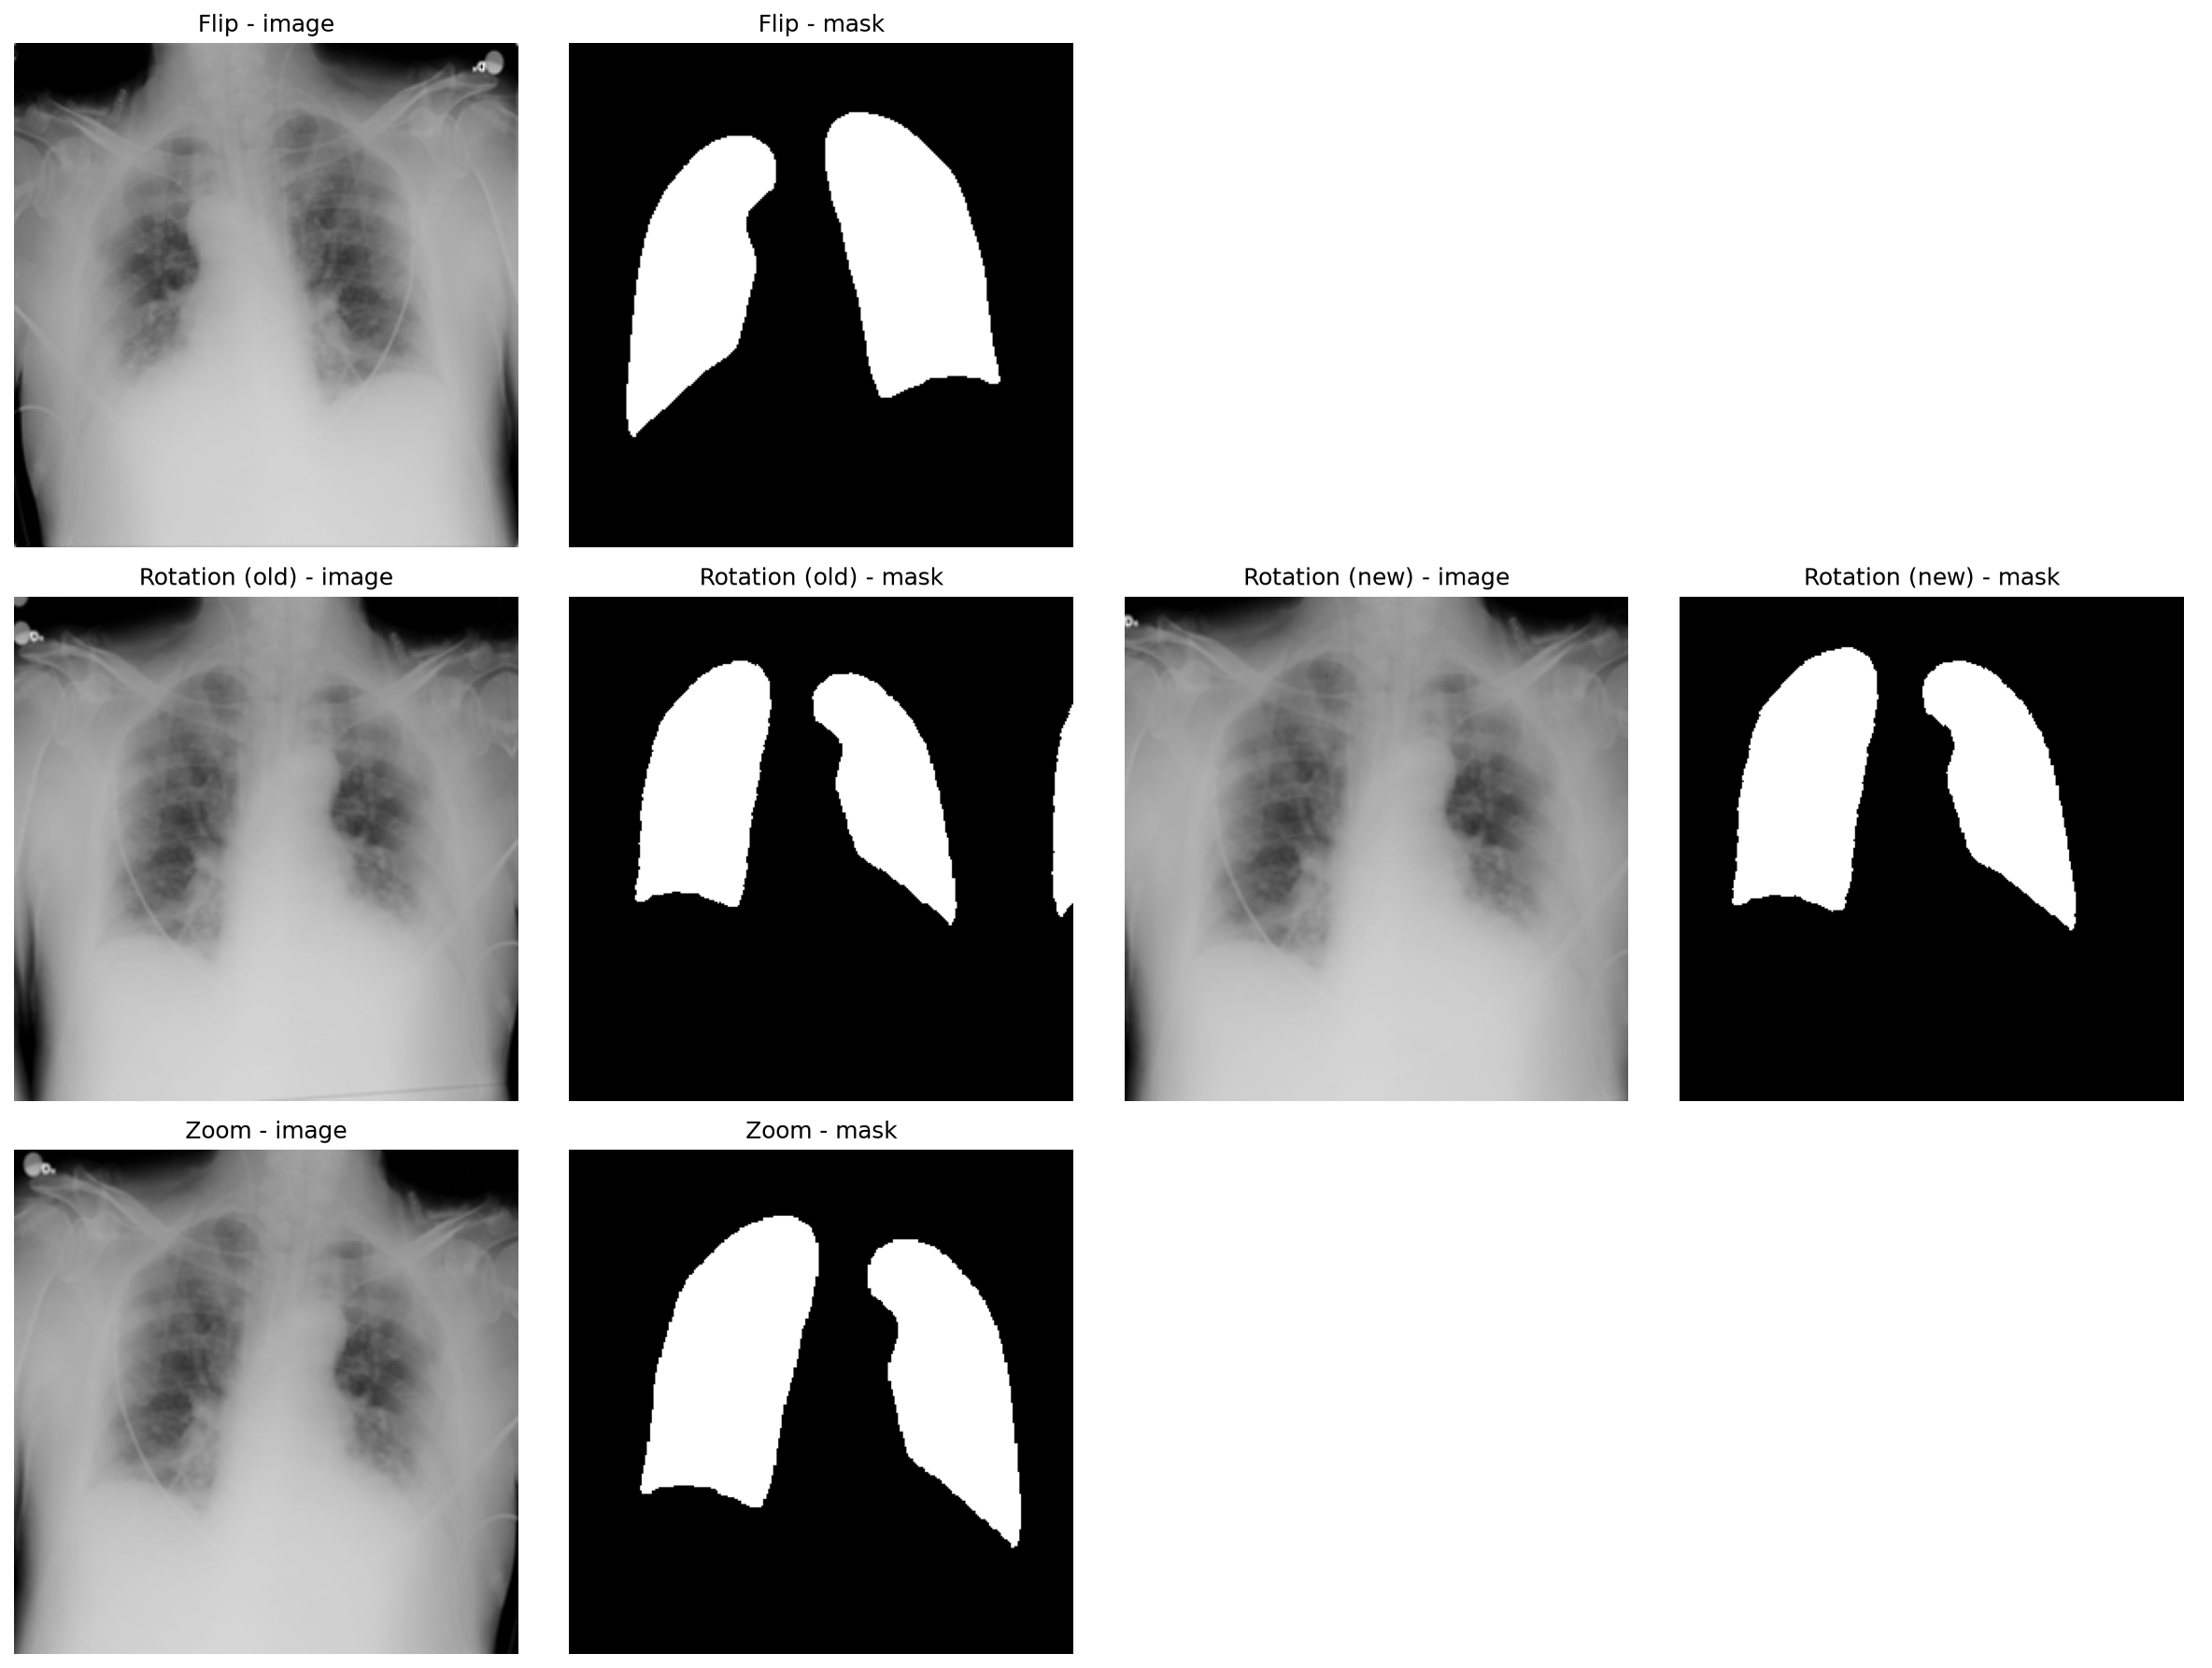
\includegraphics[width=\textwidth]{figures/preprocessing_augmentation_ops.png}
    \caption{Individual augmentation operations on a representative COVID-19 chest X-ray: horizontal flip, rotation without zoom compensation, rotation with zoom compensation, and random zoom. Each row pairs the transformed image with its aligned lung mask.}
    \label{fig:preprocessing_augmentation_ops}
\end{figure}

\begin{figure}[H]
    \centering
    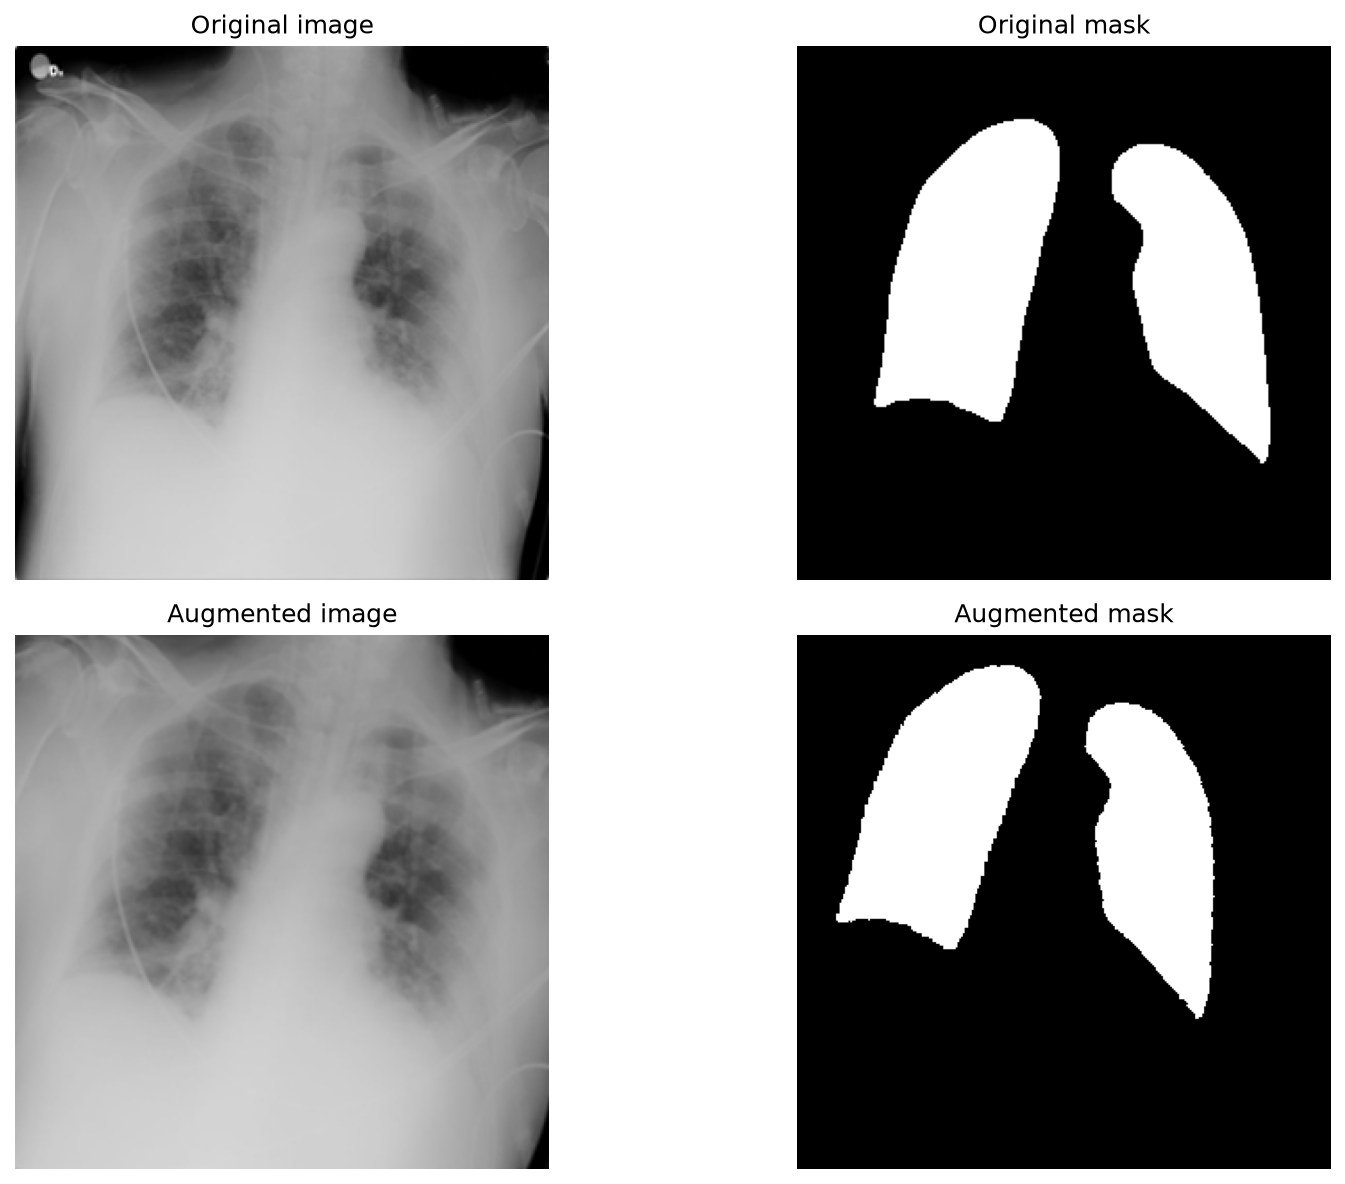
\includegraphics[width=0.85\textwidth]{figures/preprocessing_augment_pair.png}
    \caption{Original COVID-19 chest X-ray and lung mask compared with one stochastic augmentation pass (fixed random seed for reproducibility).}
    \label{fig:preprocessing_augment_pair}
\end{figure}

\section{Verification and Reproducibility}

The preprocessing workflow was verified at three levels before model training.

First, \textbf{transform correctness} was confirmed on synthetic images:
normalized outputs lie in $[0, 1]$, repeated processing without augmentation
yields identical results, lung masking zeroes non-pulmonary regions, and CLAHE
changes pixel values while preserving spatial dimensions. Geometric augmentation
preserves image and mask shape across 25 consecutive stochastic draws.

Second, \textbf{split integrity} was confirmed: the three partitions are disjoint,
together they account for all 21{,}106 retained samples, and class proportions
match the full dataset within 0.05 percentage points.

Third, \textbf{end-to-end consistency} was confirmed on the full dataset:
all 21{,}106 images were read successfully with zero failures; processed image
counts, split totals, and stacked sample counts all equal 21{,}106; and a
complete rebuild of the baseline configuration produced bit-identical outputs
to the saved training, validation, and test partitions
(14{,}774 + 3{,}166 + 3{,}166 = 21{,}106).

A total of 78 automated checks covering transforms, augmentation, splitting,
and pipeline regression passed. Stochastic steps used random seed 42 throughout.

\section{Implications for Model Development}

This preprocessing stage establishes a fixed, auditable baseline for convolutional
network training. Stratified splitting and duplicate removal reduce leakage risk;
grayscale standardization and per-image normalization target the technical shortcuts
documented in Chapter~\ref{chap:data}. Because class imbalance persists after
splitting---Viral Pneumonia remains at 6.34\% of the training set---downstream
evaluation must report per-class precision, recall, macro-averaged F1, balanced
accuracy, and confusion matrices rather than overall accuracy alone.

Optional CLAHE, lung masking, and augmentation remain available for systematic
comparison in subsequent experiments. Their impact on classification performance
and on whether the model attends to pulmonary rather than acquisition-related
features will be assessed during model development.
